% A3 @ MICRO 2026 poster, 36 in x 48 in portrait. Build: pdflatex poster.tex
% Numbers trace to the paper (circt_micro_a3_2026-2.pdf) unless a comment says otherwise.
\RequirePackage{fix-cm}
\documentclass{article}
\usepackage[paperwidth=36in,paperheight=48in,margin=0.9in]{geometry}
\usepackage[T1]{fontenc}
\usepackage{tgheros,textcomp}
\renewcommand*\familydefault{\sfdefault}
\renewcommand*\ttdefault{txtt}
\usepackage{amsmath,xcolor,tikz,pgfplots,qrcode,tcolorbox,enumitem}
\usetikzlibrary{shapes.geometric,arrows.meta,calc}
\pgfplotsset{compat=1.18,/pgf/number format/assume math mode=true}
\pagestyle{empty}
\setlength{\parindent}{0pt}

% palette: the paper's hues
\definecolor{ink}{HTML}{1F2328}
\definecolor{mute}{HTML}{55595F}
\definecolor{agF}{HTML}{EDE6F8}\definecolor{agB}{HTML}{6B4FA0}
\definecolor{rbB}{HTML}{2F6FAF}
\definecolor{dsB}{HTML}{8E8E96}
\definecolor{hgB}{HTML}{3E6B52}
\color{ink}

\newcommand{\body}{\fontsize{31}{41}\selectfont}
\renewcommand{\small}{\fontsize{27}{35}\selectfont}
\renewcommand{\tiny}{\fontsize{24}{31}\selectfont}
\newcommand{\mono}{\fontsize{26}{34}\selectfont\ttfamily}
\newcommand{\sect}[2]{\par{\fontsize{54}{62}\selectfont\bfseries\color{agB}#1\hspace{0.4em}\color{ink}#2\par}%
  \nointerlineskip\vspace{0.14in}{\color{agB}\hrule height 5pt}\vspace{0.02in}}
\newcommand{\code}[1]{\texttt{#1}}
\setlist[itemize]{leftmargin=0.9em,itemsep=0.12in,parsep=0in,topsep=0in,label={\color{agB}\textbullet}}
% column: minipage resets paragraph settings, so restore them here
\newenvironment{col}[1]{\begin{minipage}[t]{#1}\raggedright\body\setlength{\parskip}{0.22in}}{\end{minipage}}
\newcommand{\colW}{10.87in}
\newcommand{\rowgap}{\par\vspace{0.42in}}

\begin{document}\body\raggedright\frenchspacing

% ================================================================ header
\begin{col}{27.8in}
{\fontsize{30}{36}\selectfont\bfseries\color{mute}A\textsuperscript{3} WORKSHOP @ MICRO 2026 \hspace{0.3em}\textperiodcentered\hspace{0.3em} CHIA HACKATHON\par}
\vspace{0.1in}
{\fontsize{96}{110}\selectfont\bfseries From Mined Fixes to Gated Repair:\\Closed-Loop Defect Synthesis for CIRCT\par}
\vspace{0.1in}
{\fontsize{44}{54}\selectfont Abhinav Venkata Kota,\ \ Adithya Jillellamudi,\ \ Priyesh Shukla\par}
\vspace{-0.15in}
{\fontsize{30}{40}\selectfont\color{mute}IIIT Hyderabad\hspace{0.5em}\textperiodcentered\hspace{0.5em}\{abhinav.kota, adithya.jillellamudi\}@students.iiit.ac.in,\ \ priyesh.shukla@iiit.ac.in\par}
\end{col}\hfill
\begin{col}{5.4in}\centering
\vspace{0.05in}
\qrcode[height=4.1in]{https://github.com/DevAbhinav-23/CHIA_Hackathon_2k26}\par
\vspace{-0.1in}
{\small\bfseries Code, corpus, every verdict\par}
\end{col}

\rowgap
% ================================================================ hero
\begin{tcolorbox}[colback=agF,colframe=agF,arc=0.25in,boxrule=0pt,left=0.7in,right=0.6in,top=0.35in,bottom=0.35in]
\begin{minipage}[c]{20.2in}\raggedright
{\fontsize{54}{68}\selectfont\bfseries An agent that reads past compiler fixes wrote inputs that exposed fifteen new CIRCT bugs.\par}
\vspace{0.25in}
{\fontsize{40}{52}\selectfont\color{mute}Mutating the same tests found 2, from 150 times as many inputs.\par}
\vspace{0.25in}
{\fontsize{30}{40}\selectfont\color{mute}\textbf{New:} reproduced on a second worker, reduced, and matching no known issue. None is filed or maintainer-confirmed yet.\par}
\end{minipage}\hfill
\begin{minipage}[c]{11.6in}\centering
{\fontsize{44}{50}\selectfont\bfseries new bugs\par}
\vspace{-0.1in}
\begin{tabular}{@{}c@{\hspace{1.1in}}c@{}}
{\fontsize{210}{190}\selectfont\bfseries\color{agB}15} & {\fontsize{210}{190}\selectfont\bfseries\color{dsB}2}\\[0.2in]
\parbox[t]{5.2in}{\centering\fontsize{34}{42}\selectfont\bfseries reading fixes\\\mdseries\color{mute}758 inputs} &
\parbox[t]{5.2in}{\centering\fontsize{34}{42}\selectfont\bfseries mutating tests\\\mdseries\color{mute}115,869 inputs}
\end{tabular}
\end{minipage}
\end{tcolorbox}

\rowgap
% ================================================================ row A
\begin{col}{13.2in}
\sect{1}{Bugs nobody reports}
\textbf{CIRCT} is an open-source compiler for hardware, built on MLIR\,[1]. It lowers a circuit in FIRRTL or SystemVerilog to Verilog. A crash stops the designer; wrong Verilog can reach a chip.

\textbf{CHIA}\,[2], the agent framework this hackathon builds on, already repairs reported CIRCT issues. Its bottleneck is supply. Bug-labelled issues:

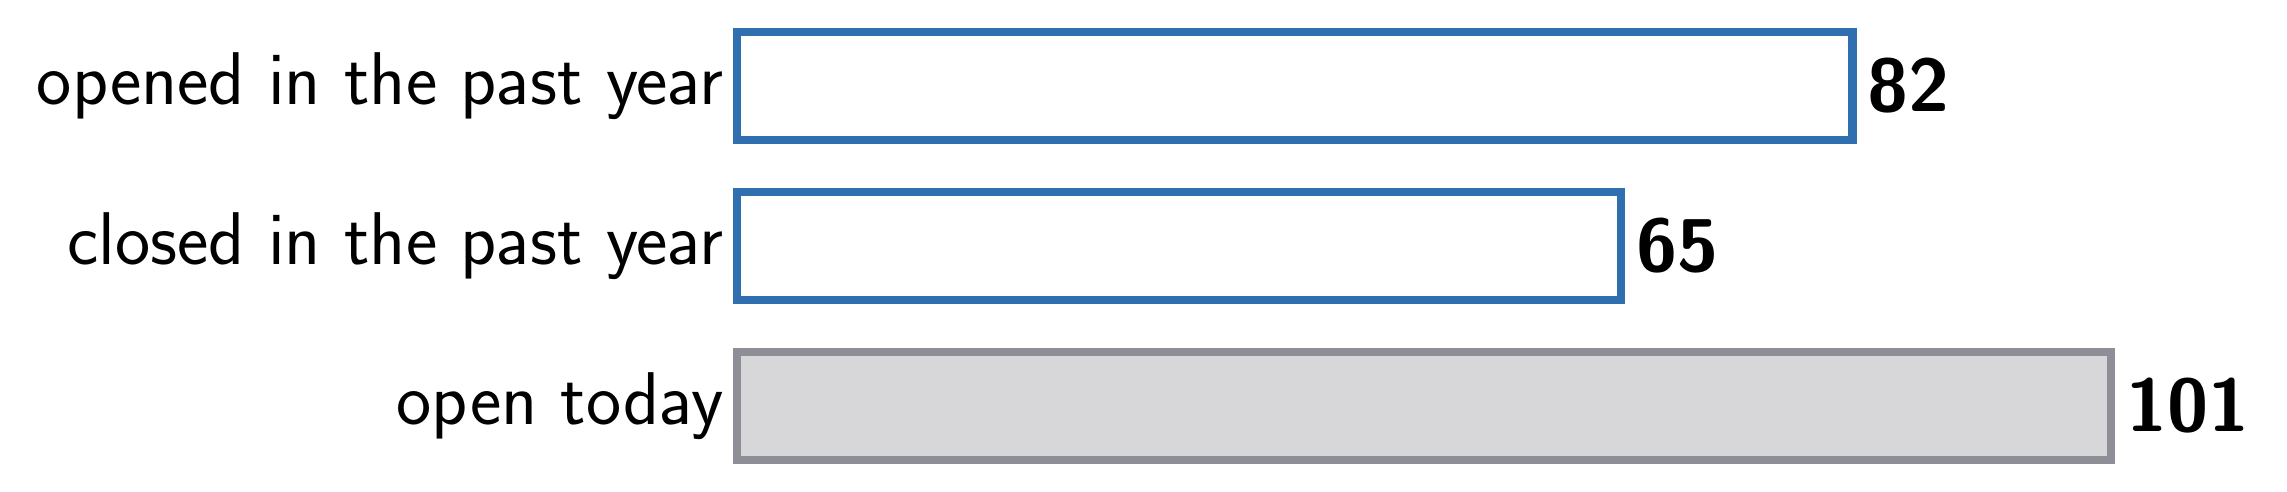
\begin{tikzpicture}[x=0.068in,y=1in,font=\small]
\foreach \y/\n/\v/\f/\d in {0/opened in the past year/82/white/rbB,-0.8/closed in the past year/65/white/rbB,-1.6/open today/101/dsB!35/dsB} {
  \node[anchor=east] at (-0.3,\y) {\n};
  \fill[\f,draw=\d,line width=3pt] (0,\y-0.27) rectangle (\v,\y+0.27);
  \node[anchor=west,font=\small\bfseries] at (\v+0.4,\y) {\v};}
\end{tikzpicture}

\vspace{-0.1in}
{\small\color{mute}The open ones have a median age of 911 days.\par}
\end{col}\hfill
\begin{col}{19.9in}
\sect{2}{A fix points at its siblings}
A past fix corrects one wrong assumption at one site; the same assumption often survives at sibling sites. The agent reads a fix and its test, names the root-cause class, and writes inputs aimed at the siblings. The idea follows AFuzz\,[4]. New here: tools, not the model, give every verdict; assertions restored; a pre-registered baseline; all as CHIA nodes.

\begin{tcolorbox}[colback=white,colframe=agB,arc=0.15in,boxrule=4pt,left=0.45in,right=0.4in,top=0.28in,bottom=0.28in]
\raggedright
{\small\textbf{\color{agB}Seed:}\ an August 2026 fix to an out-of-bounds \code{moore.extract}, the SystemVerilog slice.\par}
\vspace{0.16in}
{\small\textbf{\color{agB}The loop wrote,}\ after reduction (function wrapper omitted):\par}
\vspace{0.08in}
{\mono
\%0 = moore.array\_create \%arg0, \%arg0 : !moore.i32, !moore.i32 -> array<2 x i32>\\
\%1 = moore.extract \%0 from {\color{agB}\bfseries-2147483648} : array<2 x i32> -> array<4 x i32>\par}
\vspace{0.16in}
{\small\textbf{\color{agB}CIRCT}\ (\code{circt-opt -{}-convert-moore-to-core}) stops:\par}
\vspace{0.08in}
{\mono HWOps.cpp:1995: ArrayConcatOp::build: Assertion\\
\textasciigrave!values.empty() \&\& "Cannot build array of zero elements"\textquotesingle\ failed.\par}
\end{tcolorbox}
\end{col}
% reproducer: ~/bugloop-artefacts/f1e4fef5.../probe_p-a2cb61b8d0aa/{reduced.mlir,argv.json,stderr.txt}

\rowgap
% ================================================================ loop figure
\sect{3}{The loop: the model writes, tools decide}
\newcommand{\card}[6]{% #1 i, #2 style, #3 tag, #4 title, #5 text, #6 text colour
  \node[#2,text=#6] (c#1) at ({2.6+4.02*#1},8.4) {\parbox[t][2.95in][t]{3.0in}{\centering
    {\tiny\bfseries\color{#6!65!white}#3\par}\vspace{0.08in}
    {\fontsize{29}{35}\selectfont\bfseries #4\par}\vspace{0.1in}
    {\fontsize{25}{31}\selectfont #5\par}}};}
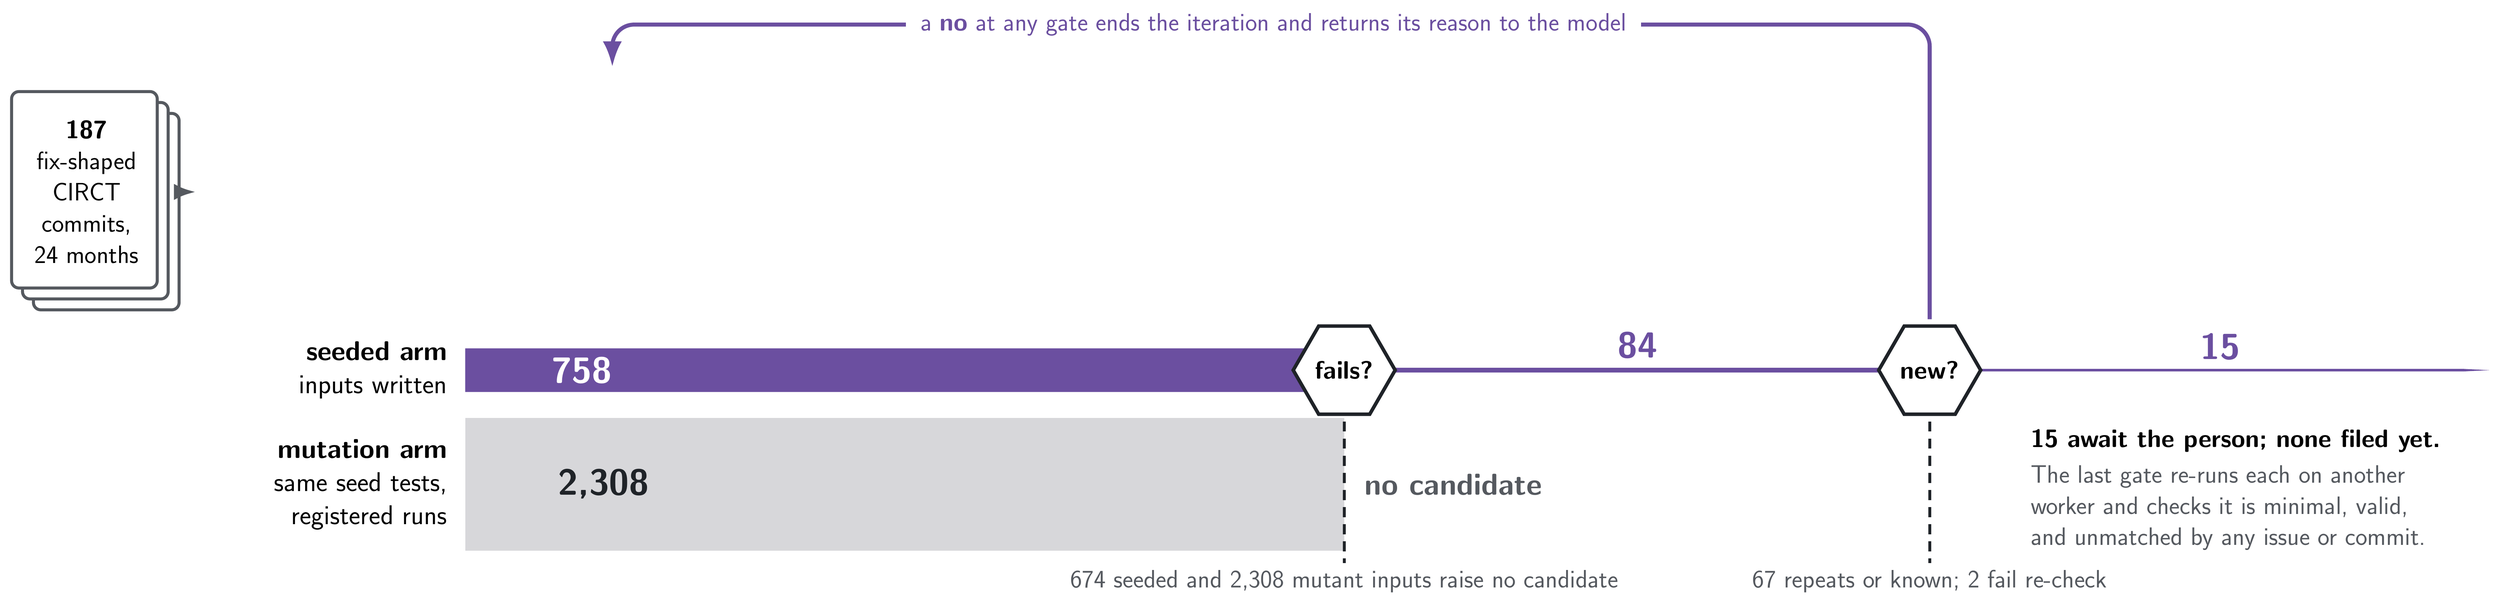
\begin{tikzpicture}[x=1in,y=1in,
  card/.style={draw,line width=4pt,rounded corners=0.14in,anchor=north west,inner sep=0.2in},
  model/.style={card,fill=agF,draw=agB},
  tool/.style={card,fill=white,draw=rbB},
  chia/.style={card,fill=white,draw=agB,dash pattern=on 14pt off 8pt},
  person/.style={card,fill=hgB,draw=hgB},
  gate/.style={regular polygon,regular polygon sides=6,draw=ink,fill=white,line width=3.5pt,inner sep=0in,font=\fontsize{25}{28}\selectfont\bfseries,minimum size=1.4in}]
% corpus
\foreach \d in {0.3,0.15,0} \node[draw=mute,fill=white,line width=3pt,rounded corners=0.1in,minimum width=2.0in,minimum height=2.7in,anchor=north west] at (0.05+\d,8.1-\d) {};
\node[align=center,font=\fontsize{25}{31}\selectfont,text width=1.8in] at (1.1,6.7) {\textbf{187}\\fix-shaped CIRCT commits, 24 months};
\draw[-{Latex[length=0.3in]},line width=4pt,mute] (2.3,6.7) -- (2.6,6.7);
% stages
\card{0}{model}{MODEL}{1\ Read a fix}{One past fix: diff and test. Name the root cause and sibling sites.}{ink}
\card{1}{model}{MODEL}{2\ Write inputs}{Aimed at the siblings, in the language of the seed's own test.}{ink}
\card{2}{tool}{TOOL}{3\ Build}{CIRCT with its assertions back on.}{ink}
\card{3}{tool}{TOOL}{4\ Judge}{Crash, assertion, or CIRCT's verifier rejects its own output.}{ink}
\card{4}{tool}{TOOL}{5\ Reduce}{\code{circt-reduce} shrinks the failing input.}{ink}
\card{5}{model}{TOOLS + MODEL}{6\ Triage}{Tools dedupe against 2,652 issues; the model writes the report.}{ink}
\card{6}{chia}{CHIA AGENT}{7\ Repair}{CHIA's issue solver drafts a patch. Tried once: no fix yet.}{ink}
\card{7}{person}{PERSON}{File}{A named author approves each filing. Default: file nothing.}{white}
% ribbons: width = 0.6 in per 758 inputs (linear); 15 drawn at a 0.034 in minimum
\def\yS{4.25}\def\yM{2.68}
\fill[agB] (6.3,\yS+0.3) -- (17.9,\yS+0.3) .. controls (18.37,\yS+0.3) and (18.37,\yS+0.033) .. (18.85,\yS+0.033)
  -- (25.95,\yS+0.033) .. controls (26.41,\yS+0.033) and (26.41,\yS+0.017) .. (26.9,\yS+0.017) -- (33.75,\yS+0.017)
  -- (34.1,\yS) -- (33.75,\yS-0.017) -- (26.9,\yS-0.017) .. controls (26.41,\yS-0.017) and (26.41,\yS-0.033) .. (25.95,\yS-0.033)
  -- (18.85,\yS-0.033) .. controls (18.37,\yS-0.033) and (18.37,\yS-0.3) .. (17.9,\yS-0.3) -- (6.3,\yS-0.3) -- cycle;
\fill[dsB!35] (6.3,\yM+0.914) rectangle (18.37,\yM-0.914);
\node[font=\fontsize{36}{40}\selectfont\bfseries,text=white] at (7.9,\yS) {758};
\node[font=\fontsize{36}{40}\selectfont\bfseries,text=ink] at (8.2,\yM) {2,308};
\node[font=\fontsize{36}{40}\selectfont\bfseries,text=agB,anchor=south] at (22.4,\yS+0.12) {84};
\node[font=\fontsize{36}{40}\selectfont\bfseries,text=agB,anchor=south] at (30.4,\yS+0.1) {15};
\node[anchor=east,align=right,font=\fontsize{27}{33}\selectfont] at (6.1,\yS) {\textbf{seeded arm}\\inputs written};
\node[anchor=east,align=right,font=\fontsize{27}{33}\selectfont] at (6.1,\yM) {\textbf{mutation arm}\\same seed tests,\\registered runs};
% gates with counted losses sit on the ribbon; the mutation ribbon stops at the first
\foreach \x/\q in {18.37/fails?,26.41/new?} {
  \draw[line width=3pt,ink,dash pattern=on 10pt off 7pt] (\x,\yS) -- (\x,1.6);
  \node[gate] at (\x,\yS) {\q};}
\node[anchor=west,font=\fontsize{30}{36}\selectfont\bfseries,text=mute] at (18.6,\yM) {no candidate};
\node[anchor=north,align=center,font=\fontsize{25}{31}\selectfont,text=mute] at (18.37,1.55) {674 seeded and 2,308 mutant inputs raise no candidate};
\node[anchor=north,align=center,font=\fontsize{25}{31}\selectfont,text=mute] at (26.41,1.55) {67 repeats or known; 2 fail re-check};
\node[anchor=north west,align=left,font=\fontsize{25}{31}\selectfont] at (27.75,\yM+0.8) {\textbf{15 await the person; none filed yet.}\\[0.06in]
  \color{mute}The last gate re-runs each on another\\\color{mute}worker and checks it is minimal, valid,\\\color{mute}and unmatched by any issue or commit.};
% feedback rail from the last tool gate back to stage 2
\draw[line width=4pt,agB,-{Latex[length=0.35in]},rounded corners=0.3in] (26.41,4.95) -- (26.41,9.0) -- (8.32,9.0) -- (8.32,8.42);
\node[fill=white,inner xsep=0.2in,font=\fontsize{25}{30}\selectfont\color{agB}] at (17.4,9.0) {a \textbf{no} at any gate ends the iteration and returns its reason to the model};
\end{tikzpicture}

\vspace{0.15in}
{\small\color{mute}One model (Gemini 3.8 Flash, through CHIA) acts only in MODEL stages; tools answer every gate. Ribbon width is proportional to count, both campaigns summed; the 15 is drawn at a minimum width.\par}

\rowgap
% ================================================================ row B
\begin{col}{\colW}
\sect{4}{A fair test}
\begin{itemize}
\item Both arms share harness, oracles, reducer and gate; only the generator differs.
\item Mutation arm: seed tests rewritten without the fix, after Mut4All\,[3]; 1,154 mutants from 96 seeds per campaign, no model.
\item Registered runs: the mutation arm used up its mutants in minutes. Given the whole window later, it gated 2 bugs (12 vs 2 over \textasciitilde12\,h, different hardware).
\item Dedup errs on 1 of 11 distinct and 1 of 11 duplicate labelled pairs.
\end{itemize}
\end{col}\hfill
\begin{col}{\colW}
\sect{5}{A consistent rate}
Per 100 inputs, campaigns about five times apart in size agree. Fifteen bugs show a consistent rate, not an effect size.

\vspace{-0.05in}
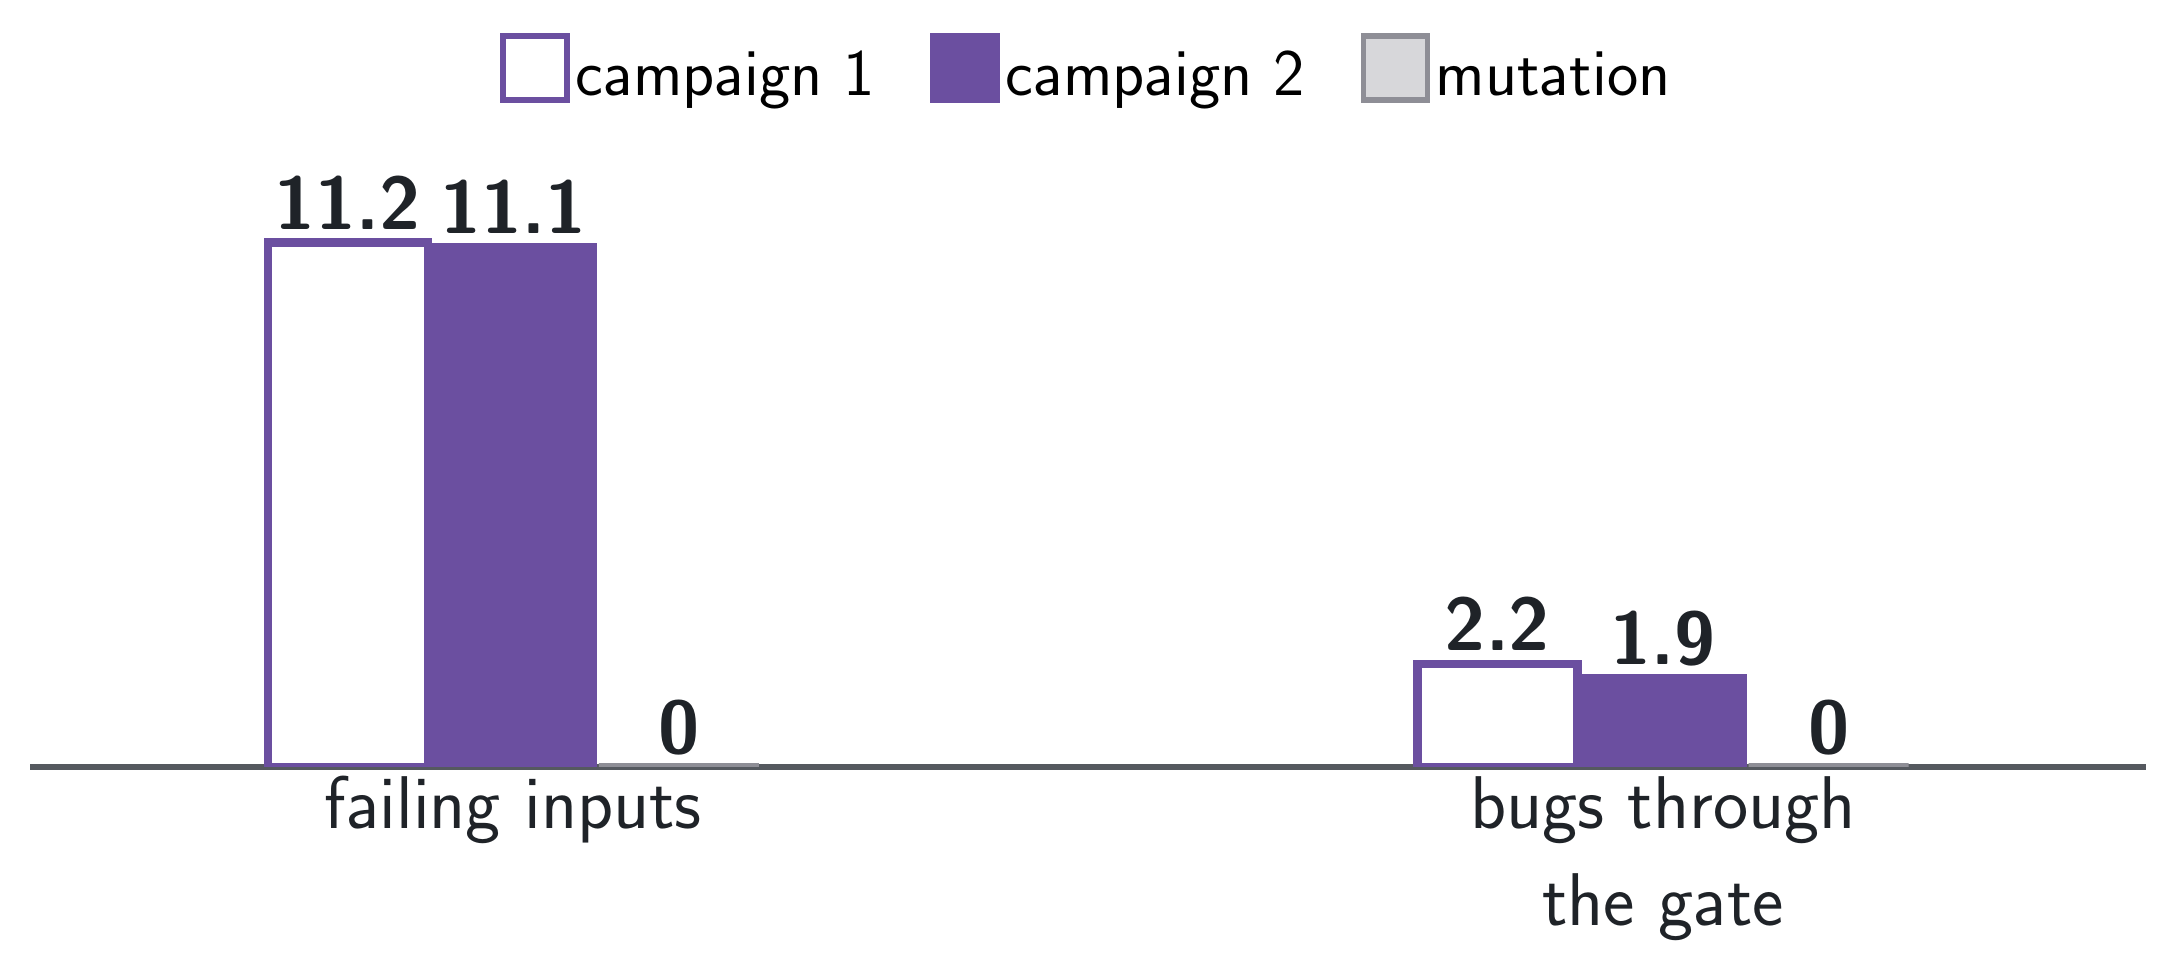
\begin{tikzpicture}
\begin{axis}[ybar,width=11.2in,height=3.9in,bar width=0.8in,ymin=0,ymax=14,
  axis x line*=bottom,axis y line=none,enlarge x limits=0.42,
  symbolic x coords={fail,gate},xtick=data,
  xticklabels={{failing inputs},{bugs through\\the gate}},
  xticklabel style={font=\small,align=center,text=ink},
  nodes near coords,every node near coord/.append style={font=\small\bfseries,text=ink},
  axis line style={mute,line width=2pt},major tick length=0pt,
  legend style={font=\tiny,draw=none,fill=none,at={(0.5,1.0)},anchor=south,legend columns=-1,/tikz/every even column/.append style={column sep=0.25in}},
  legend image code/.code={\draw[#1,line width=2pt] (0in,-0.12in) rectangle (0.32in,0.2in);}]
\addplot[fill=white,draw=agB,line width=3pt] coordinates {(fail,11.2) (gate,2.2)};
\addplot[fill=agB,draw=agB,line width=3pt] coordinates {(fail,11.1) (gate,1.9)};
\addplot[fill=dsB!35,draw=dsB,line width=3pt] coordinates {(fail,0) (gate,0)};
\legend{campaign 1,campaign 2,mutation}
\end{axis}
\end{tikzpicture}

\vspace{-0.1in}
{\tiny\color{mute}Campaign 1: 9 seeds, 134 inputs. Campaign 2: 43 seeds, 624 inputs. USD 14.8 and 10.2 per gated bug at list price.\par}
\end{col}\hfill
\begin{col}{\colW}
\sect{6}{Fifteen new bugs}
Three from the seed in box 2; twelve across the compiler, three of them not assertions at all. Examples:
\begin{itemize}
\item zero-element array: assertion at \code{HWOps.cpp:1995}
\item \code{comb.extract}, \code{llhd.sig.extract} emitted with aggregate types; CIRCT's own verifier rejects them
\item segfault in \code{resolveClassStructBody}, \code{MooreToCore.cpp}
\item abort in \code{ElaboratedObjectOp::\allowbreak verifySymbolUses}, \code{OMOps.cpp}
\end{itemize}
\end{col}

\rowgap
% ================================================================ row C
\begin{col}{\colW}
\sect{7}{What it took}
\textbf{Rebuild the past in minutes:} prebuilt LLVM SDKs match the pin of 171 of 187 seeds, so no hours-long LLVM build.

\textbf{Let the compiler complain:} CHIA's image compiles CIRCT's assertions out. \code{-UNDEBUG} restores them in every object that asserts (536 of 555); the same 1,119 tests pass.
\end{col}\hfill
\begin{col}{\colW}
\sect{8}{Not claimed}
\begin{itemize}
\item No maintainer has confirmed these bugs; none is filed yet.
\item 43 of 187 seeds ran, at 3.6 seeds an hour on Vertex.
\item No fix: the repair chain's one patch was a debug print.
\item Wrong-output bugs are only reported.
\end{itemize}
\end{col}\hfill
\begin{col}{\colW}
\sect{9}{Take it}
The loop as CHIA nodes and tools, with 736 tests; the corpus; every input, verdict, reduced case and transcript. Ready for CHIA upstream, not yet submitted: the assertions-on image and its build.

{\fontsize{25}{32}\selectfont\ttfamily github.com/DevAbhinav-23/CHIA\_Hackathon\_2k26\par}

{\tiny\color{mute}We thank the CHIA developers and the A\textsuperscript{3} organisers. Claude (Anthropic) helped draft text, code and this poster; the authors answer for every claim.\par}
\end{col}

\vfill
{\color{dsB}\hrule height 2pt}\vspace{0.2in}
{\tiny\color{mute}[1] C.\,Lattner et al., ``MLIR,'' CGO 2021.\quad [2] A.\,Cui et al., ``CHIA,'' arXiv:2606.27350, 2026.\quad [3] B.\,Wang et al., ``Mut4All,'' arXiv:2507.19275, 2025.\quad [4] J.\,Park, I.\,Yun, ``Agentic fuzzing,'' arXiv:2605.10074, 2026.\par}

\end{document}
